\documentclass[11pt, fleqn]{article}

\usepackage{amsmath}
\usepackage{amsfonts}
\usepackage{amsthm}
\usepackage[margin=1in]{geometry} % To set the margin widths
\usepackage{graphicx}
%\usepackage{hyperref}
\usepackage{listings}
\usepackage{multirow}
\usepackage{tabularx}
\usepackage{varioref}
\usepackage{cleveref}  % this redefines vref to use cleverref
\usepackage{siunitx}
%\usepackage{subcaption}
\usepackage{subfig}
\usepackage{titlesec}
\usepackage{bm}

\crefname{equation}{equation}{equations}
\crefname{figure}{figure}{figures}

\sisetup{output-exponent-marker=\textsc{e}}

\titleformat{\section}[block]{\bfseries}{\thesection}{1em}{}


\setlength{\parskip}{12pt} % Sets a blank line in between paragraphs
\setlength\parindent{0pt} % Sets the indent for each paragraph to zero

\begin{document}

\title{Big Data: Homework 3}
\author{Will Clark \& Matthew DeLio \\ 41201-01}
\date{\today}
\maketitle

\section{Player Contribution Regression}

The model for player contribution is:
\[ \log\left[\frac{Pr(y=1)}{1-Pr(y=1)}\right] = \beta_0 + \alpha_{\texttt{team,season}} + \alpha_{\texttt{config}} + \sum_{\texttt{homeplyr}} \beta_j + \sum_{\texttt{awayplyr}} \beta_j \]
For a given player \textit{j}, the model estimates the odds multiplier that a goal scored while player \textit{j} is on the ice was scored by the his team. It includes the following two control factors:
\begin{itemize}
  \item \texttt{team,season}: This should control for high- or low-offense years, certain arenas that provide a special home-ice advantage, or coaches that are better/worse than average; and
  \item \texttt{config}: This should control for disproportionate playing time in power plays or end-of-game situations where the goalie has been pulled.
\end{itemize}
To use one example, the coefficient on Alex Ovechkin is 0.30. This means that a goal scored while Ovechkin is on the ice is $\exp(0.30)=1.35$ times as likely to be scored by his team, the Washington Capitals, than by their opponents. Put differently, if a goal is scored while Ovi is on the ice, it is 35 percent more likely that it is scored by the Caps than by their opponents.

We can sort the array of player coefficients to determine the 10 most and least valuable players in the data set. We show the results in Table~\ref{tab:best10} and Table~\ref{tab:worst10}. This evaluation metric accords with our intuition about hockey. The list of 10 best players includes some of the conventionally-regarded best players of the last decade, which tells us the model is doing a reasonably good job of quantifying performance. It also includes one player (Tyler Toffoli) who has only played since 2013, although his brief career has been successful to date. Table~\ref{tab:best10} and Table~\ref{tab:worst10} have a column labeled \textbf{G}, displaying the number of goals a player was on the ice for. We can see that Toffoli is indeed an inexperienced player compared to veterans like Joe Thornton and Pavel Datsyuk

By this performance metric, the best and worst players are both outliers and most players have a 0 rating. The sample includes 2439 players and only 646 have non-zero ratings (390 have net positive and 256 have net negative ratings). We can see in Figure~\ref{fig:play_rtg} that only a small handful of players are significantly better or significantly worse than average.

\begin{figure}[!htb]
  \centering
  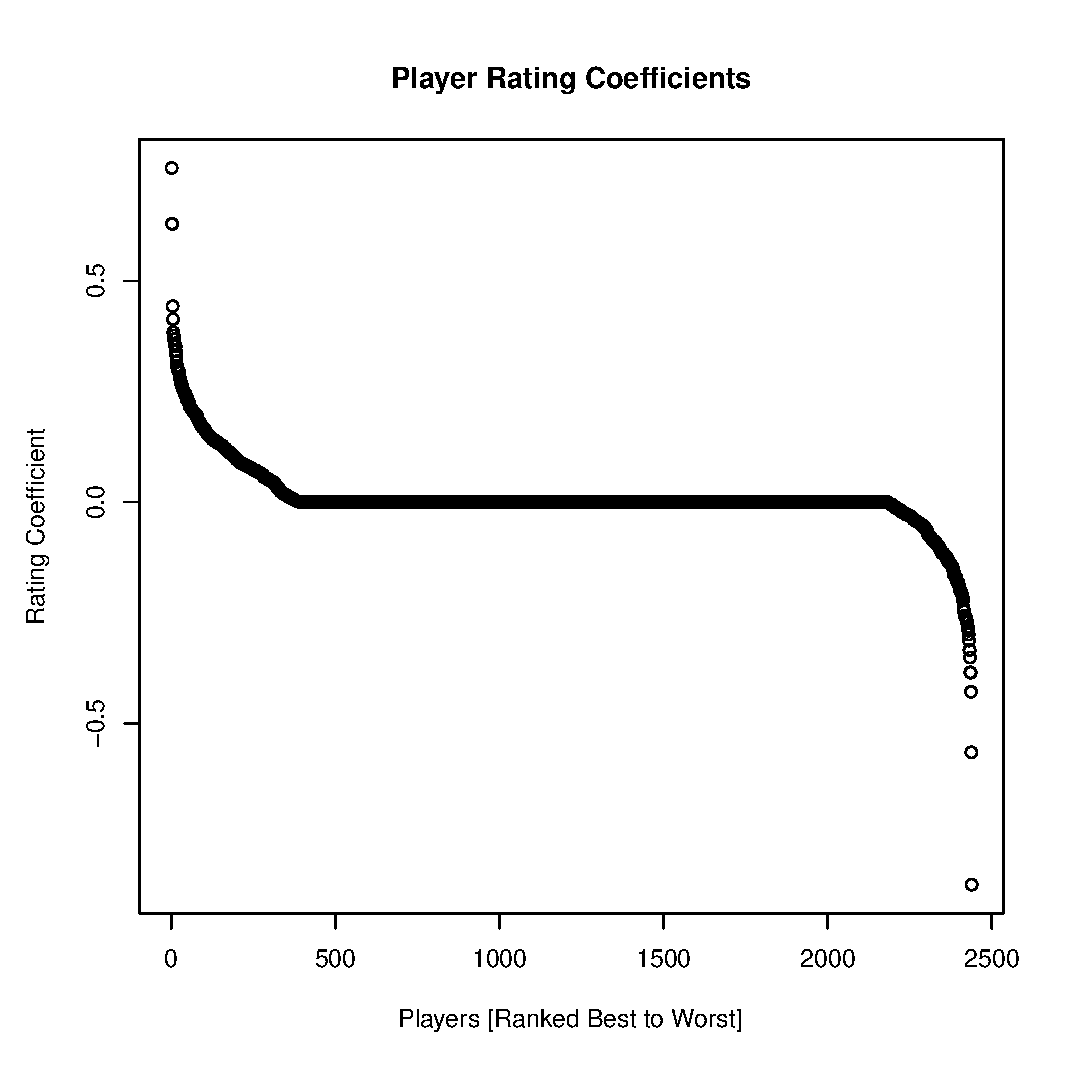
\includegraphics[scale=.5]{player_rtg.eps}
  \caption{Player Ratings Based on Regression Estimate}
  \label{fig:play_rtg}
\end{figure}

% latex table generated in R 3.0.2 by xtable 1.7-4 package
% Thu Apr 23 20:19:25 2015
\begin{table}[ht]
\centering
\begin{tabular}{rlllll}
  \hline
 & Player & Rank & $\beta_j$ & $\exp(\beta_j)$ & G \\ 
  \hline
1 & PETER FORSBERG & 1 & 0.7548 & 2.1272 & 532 \\ 
  2 & TYLER TOFFOLI & 2 & 0.6293 & 1.8762 & 93 \\ 
  3 & ONDREJ PALAT & 3 & 0.6284 & 1.8746 & 140 \\ 
  4 & ZIGMUND PALFFY & 4 & 0.4427 & 1.5569 & 197 \\ 
  5 & SIDNEY CROSBY & 5 & 0.4131 & 1.5115 & 1568 \\ 
  6 & JOE THORNTON & 6 & 0.3838 & 1.4678 & 1740 \\ 
  7 & PAVEL DATSYUK & 7 & 0.3762 & 1.4567 & 1725 \\ 
  8 & LOGAN COUTURE & 8 & 0.3682 & 1.4451 & 513 \\ 
  9 & ERIC FEHR & 9 & 0.3677 & 1.4444 & 369 \\ 
  10 & MARTIN GELINAS & 10 & 0.3578 & 1.4301 & 460 \\ 
   \hline
\end{tabular}
\caption{Top 10 NHL Players (2002-2014)} 
\label{tab:best10}
\end{table}

% latex table generated in R 3.0.2 by xtable 1.7-4 package
% Tue Apr 21 15:57:44 2015
\begin{table}[ht]
\centering
\begin{tabular}{rlllll}
  \hline
 & Player & Rank & $\beta_j$ & $\exp(\beta_j)$ & G \\ 
  \hline
1 & RYAN HOLLWEG & 2430 & -0.2989 & 0.7417 & 78 \\ 
  2 & RAITIS IVANANS & 2431 & -0.3129 & 0.7313 & 81 \\ 
  3 & DARROLL POWE & 2432 & -0.3340 & 0.7161 & 337 \\ 
  4 & CHRIS DINGMAN & 2433 & -0.3342 & 0.7159 & 30 \\ 
  5 & MATHIEU BIRON & 2434 & -0.3512 & 0.7038 & 203 \\ 
  6 & THOMAS POCK & 2435 & -0.3844 & 0.6809 & 131 \\ 
  7 & NICLAS HAVELID & 2436 & -0.3855 & 0.6801 & 1041 \\ 
  8 & P. J. AXELSSON & 2437 & -0.4284 & 0.6516 & 121 \\ 
  9 & JOHN MCCARTHY & 2438 & -0.5652 & 0.5683 & 45 \\ 
  10 & TIM TAYLOR & 2439 & -0.8643 & 0.4213 & 148 \\ 
   \hline
\end{tabular}
\caption{Bottom 10 NHL Players (2002-2014)} 
\label{tab:worst10}
\end{table}


\section{Gamma-Lasso Regression Standardization}

The Gamma-Lasso regression estimates the coefficients $\beta_j$ by minimizing an objective function similar to:
\[ \min_{\lambda} \left( -\frac{2}{n}\log \text{LHD}(\beta) + \lambda \sum_{j} c(\beta_j) \right) \]
For this discussion, we will assume that the cost function is a simple lasso of the form $c(\beta_j) = \lvert \beta_j \rvert$. In most cases we would scale this penalty function by the standard deviation of $x_j$, but doing so in this example would penalize players who have been on the ice for a large number of goals.

We ran the Gamma-Lasso regression setting \texttt{standardize=TRUE} and the resulting list of the 10 best players had been on the ice for a combined 31 goals between them. We can look more closely at two example players, Pavel Datsyuk and Jeff Toms, to see how the standardized penalty functions led to this outcome.

Datsyuk is a long-tenured player who has been on the ice for 1725 goals; he is ranked 7th by our logit regression model. Toms had a long career in the NHL and minor leagues but played his last NHL game in 2002, seeing action in only eight games and being on the ice for only four goals (which are the only four included in our data set). For Datsyuk, $\mathrm{var}(x_j)=0.0248$ while for Toms, $\mathrm{var}(x_j)=\num{5.7597e-5}$.

Figure~\ref{fig:cost_fcn} shows what the lasso penalty functions look like for each player \textit{after} they have been scaled by the standard deviation of $x_j$. We can see that there is a very high cost for the coefficient on Pavel Datsyuk and almost no cost on the coefficient for Jeff Toms. What this means for the estimation is that the coefficient on Datsyuk is very likely to be small, and the coefficient on Toms is very likely to be larger. This is in fact what we see from running the Gamma-Lasso regression setting \texttt{standardize=TRUE}; the coefficient on Datsyuk is 0.2908 while the coefficient on Toms is 1.7381.

\begin{figure}[!htb]
  \centering
  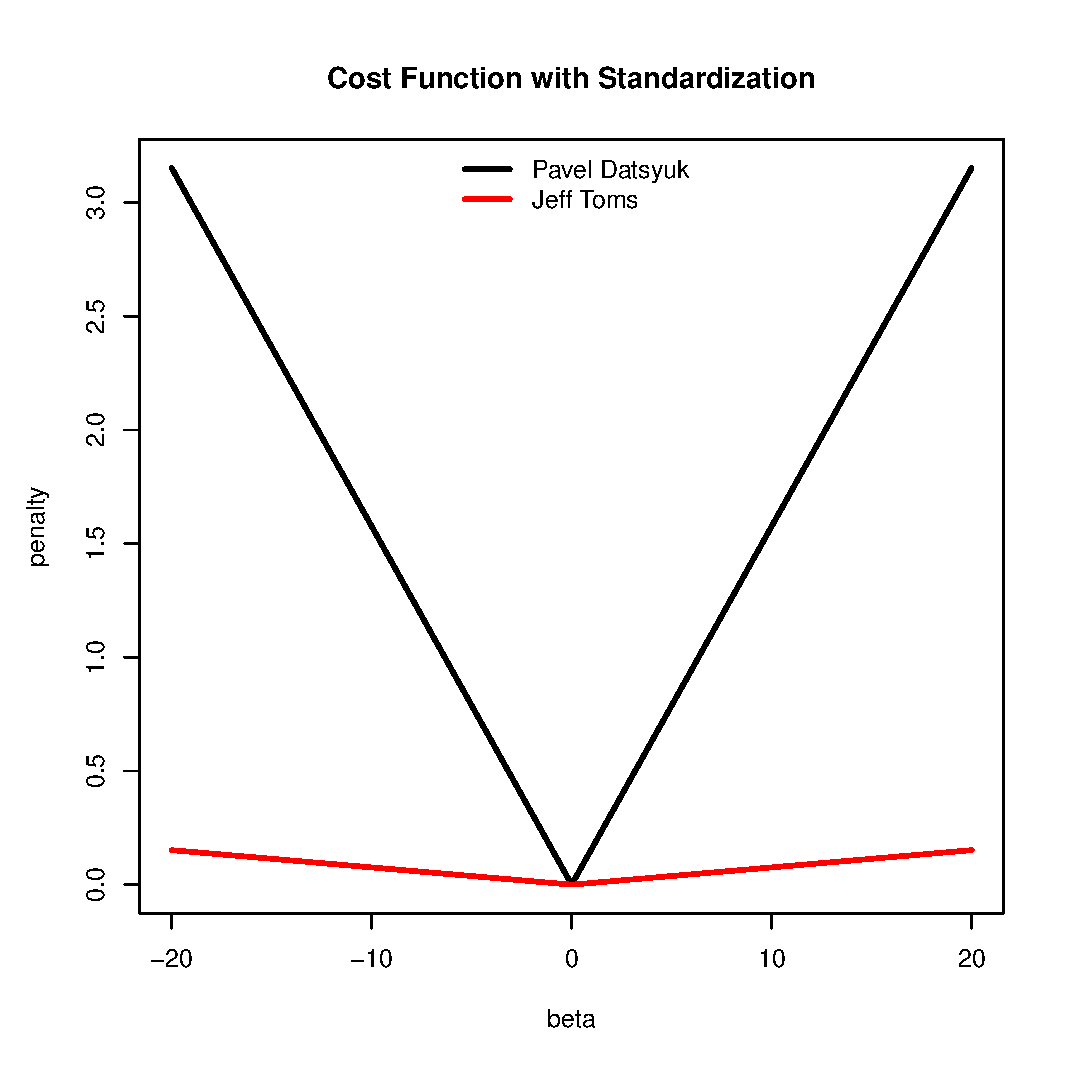
\includegraphics[scale=.5]{cost_fcn.eps}
  \caption{Lasso Cost Functions}
  \label{fig:cost_fcn}
\end{figure}

\section{IC and CV Model Selection}
\label{sec:model}

For this discussion we are looking at 3 information criteria, AIC, AICc, and BIC, used in model selection.  To compare these different criteria, we employ a 5-fold cross-validation to provide an estimate of the Out-of-Sample error (see Figure~\vref{fig:cv_nhl}).  Included on that figure is the mean-squared error for the different folds across many different values for $\lambda$.  The $\lambda$ yielding the minimum average mean-squared error as well as the largest one yielding an average MSE no more than 1 standard error away from the minimum.  Choosing the value of $\lambda_{1se}$ will yield a simpler model (i.e. one with less coefficients), but one with, potentially, a higher mean-squared error for any new data samples.

Since cross-validation is expensive (in terms of compute-time), the goal is to find another information criteria that will approximate the $\lambda$s provided by the cross-validated model.  Figure~\ref{fig:ic_nhl} shows the `gamlr' coefficient path plot with varying $\lambda$s.  The $\lambda$s that minimize AIC, AICc, and BIC as well as CV.min and CV.1se are also shown in the verticals on the plot (see Table~\vref{tab:ic} for the numerical values).  \textit{Note: In Figure~\vref{fig:ic_nhl} that AIC and AICc are almost identical therefore one is obscured by the other.}  From these data we see that both AIC/AICc do a reasonable job at estimating CV.min, opting for a more complex model (1203 vs 1113 covariates) at the expense of slightly worse MSE for new samples.  The BIC chooses a much simpler model, with far fewer coefficients than even the one prescribed by CV.1se (340 vs 634 covariates).  Because the MSE for new samples will likely be higher than that chosen by AIC and AICc, BIC is likely inferior to these other information criteria.

% latex table generated in R 3.1.2 by xtable 1.7-4 package
% Thu Apr 23 20:09:50 2015
\begin{table}[ht]
\centering
\begin{tabular}{rrr}
  \hline
 & $log(\lambda)$ & Covariates Selected \\ 
  \hline
AICc & -6.28 & 1203 \\ 
  AIC & -6.28 & 1203 \\ 
  BIC & -4.74 & 340 \\ 
  CV.Min & -6.19 & 1113 \\ 
  CV.1se & -5.67 & 604 \\ 
   \hline
\end{tabular}
\caption{ICs for NHL Data} 
\label{tab:ic}
\end{table}


\begin{figure}
  \centering
  \begin{subfigure}[b]{0.49\textwidth}
    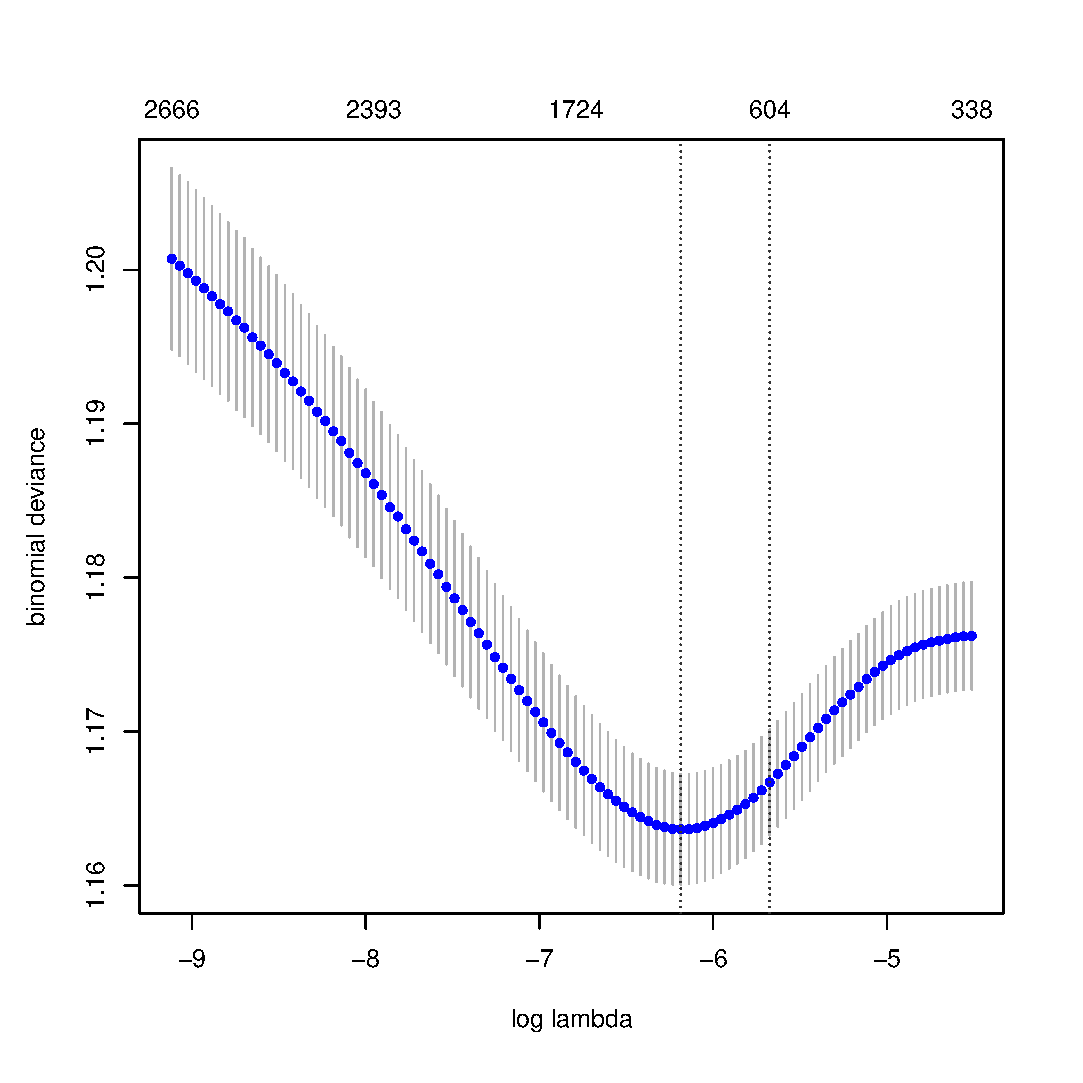
\includegraphics[width=\textwidth]{cv_nhl_gamlr_a.eps}
    \caption{CV Lasso with CV.min and CV.1se}
    \label{fig:cv_nhl}
  \end{subfigure}
  \hfill
  \begin{subfigure}[b]{0.49\textwidth}
    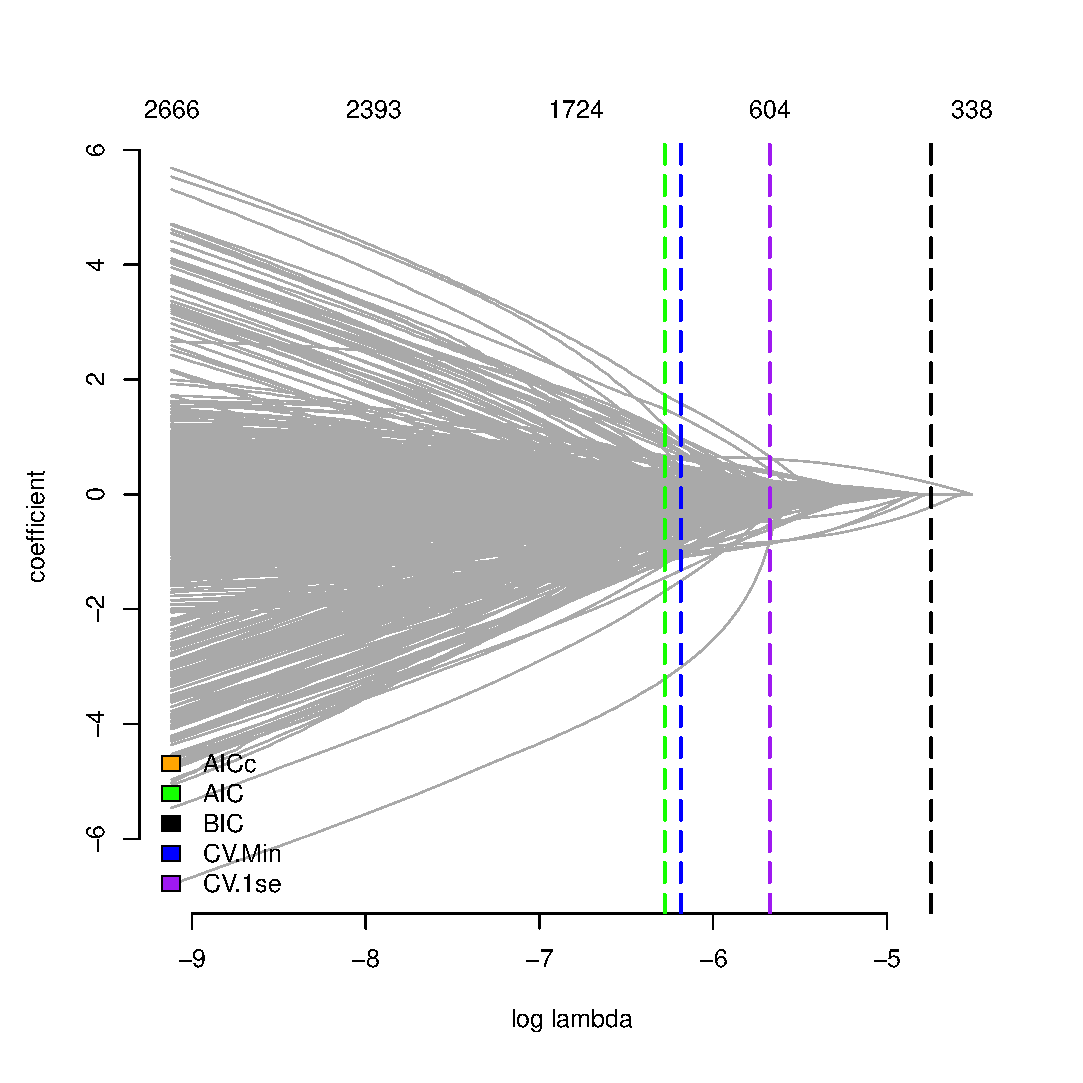
\includegraphics[width=\textwidth]{ic_nhl_c.eps}
    \caption{Gamma-Lasso Path Plot with ICs}
    \label{fig:ic_nhl}
  \end{subfigure}
  \caption{CV and Gamma Lasso Results for Complete Model}
\end{figure}

\section{Removing Team/Special Play From the Regression}

In this section we explore what happens when the team, season and special play effects are removed from the model.  Very similar to the original model, the new model is therefore governed by:

\[ \log\left[\frac{Pr(y=1)}{1-Pr(y=1)}\right] = \beta_0 + \sum_{\texttt{homeplyr}} \beta_j + \sum_{\texttt{awayplyr}} \beta_j \]

With this new model, we run the Gamma-Lasso regression as before as well as the 5-fold CV lasso.  With the default choice of $lambda.min.ratio$ we noticed that the CV average MSE never displays a minimum.  To satisfy our curiosity, we lowered this parameter to $\exp{-10}$ and re-ran the CV lasso.  After re-running it, we found a minimum at $log(\lambda)=-9.46$, a value which includes a majority of the covariates (2405 out of 2439) in the final model (see Figure~\vref{fig:pl_cv_nhl}).  Next we ran the Gamma-Lasso regression with the same $lambda.min.ratio$ and found the AIC, AICc, and BIC information criteria for the run (see Figure~\vref{fig:pl_ic_nhl} and Table~\vref{tab:pl_ic}).

To explore this further, we examine the definition of each of the information criteria (see Equations~\eqref{eq:AICc}, \eqref{eq:AIC}, \% \eqref{eq:BIC}).  As $log(lambda)$ becomes increasingly negative (adding more covariates to the model), deviance necessarily decreases.  These formulas ``penalize'' the decrease in deviance every time a new degree of freedom (new covariate) is added to the model.  To obtain minima like the ones seen in Section\ref{sec:model}, the marginal deviance for each addition degree-of-freedom must be lower than the penalty.  However, for AIC and AICc, we see no such phenomena, the penalty of adding the degree of freedom is still lower than the benefit in deviance.  Therefore these ICs estimate that the best model is the one where all covariates are included.  Indeed this seems to match closely what the CV lasso predicts as well.  For BIC, there is a clear minimum at $log(lambda)=-5.22$, which yields a simplistic model consisting of only 338 covariates.

% latex table generated in R 3.1.2 by xtable 1.7-4 package
% Wed Apr 22 14:03:05 2015
\begin{table}[ht]
\centering
\begin{tabular}{rr}
  \hline
 & $log(\lambda)$ \\ 
  \hline
AICc & -8.21 \\ 
  AIC & -8.21 \\ 
  BIC & -5.23 \\ 
  CV.Min & -8.21 \\ 
  CV.1se & -8.02 \\ 
   \hline
\end{tabular}
\caption{ICs for Player-Only Data} 
\label{tab:pl_ic}
\end{table}


Because we have the more complete (and complex) model consisting of the power-play and team statistics that shows a lower binomial deviance from far few covariates, it is clear that this simplified model suffers from omitted-variable bias.  As a result the simplified one compensates the best way it can, by including all covariates. 

\begin{equation}
  AICc = \texttt{Deviance} + 2df\frac{n}{n-df-1}
  \label{eq:AICc}
\end{equation}
\begin{equation}
  AIC = \texttt{Deviance} + 2df
  \label{eq:AIC}
\end{equation}
\begin{equation}
  BIC = \texttt{Deviance} + df * log(n)
  \label{eq:BIC}
\end{equation}

\begin{figure}
  \centering
  \begin{subfigure}[b]{0.49\textwidth}
    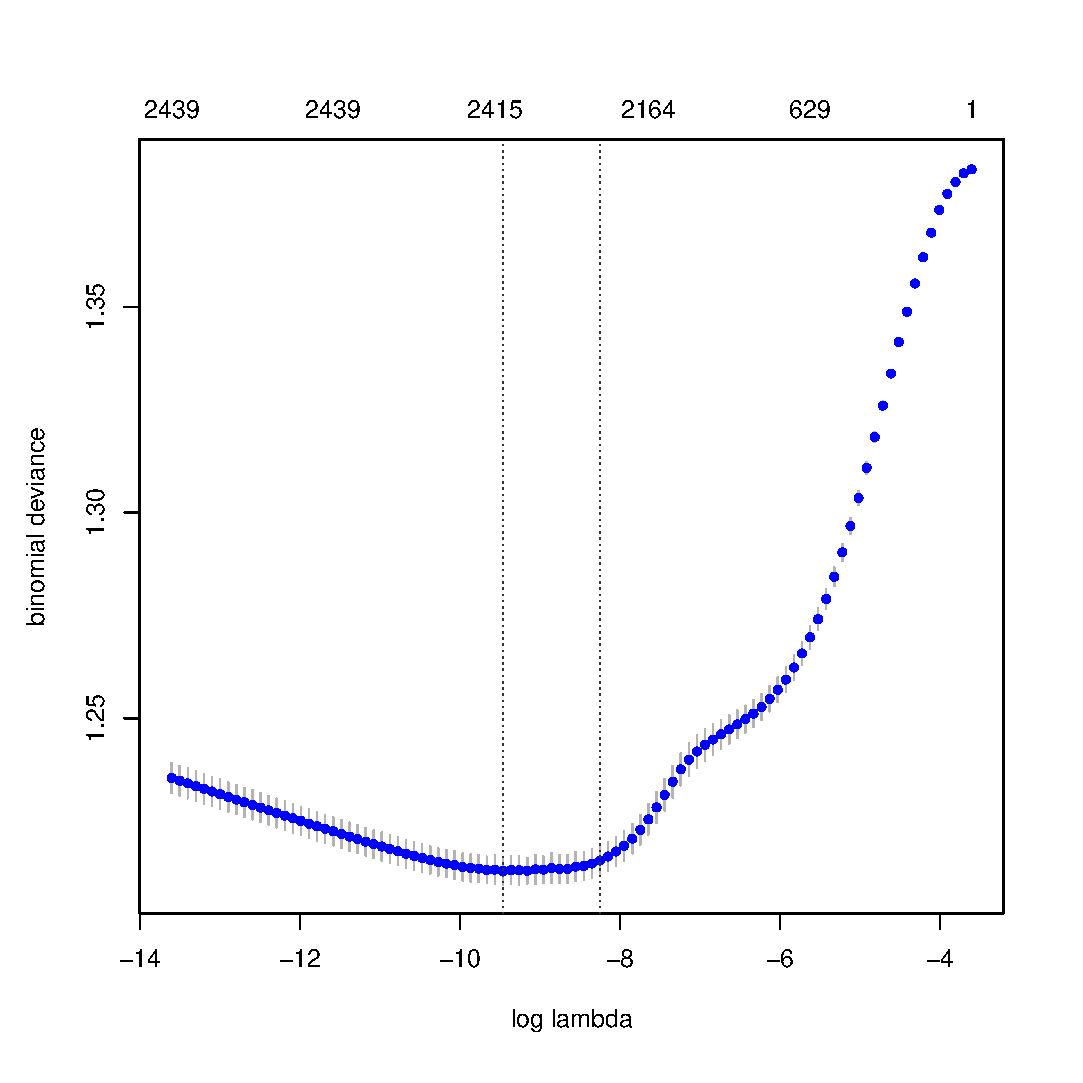
\includegraphics[width=\textwidth]{pl_cv_nhl_gamlr_a.eps}
    \caption{CV Lasso with CV.min and CV.1se}
    \label{fig:pl_cv_nhl}
  \end{subfigure}
  \hfill
  \begin{subfigure}[b]{0.49\textwidth}
    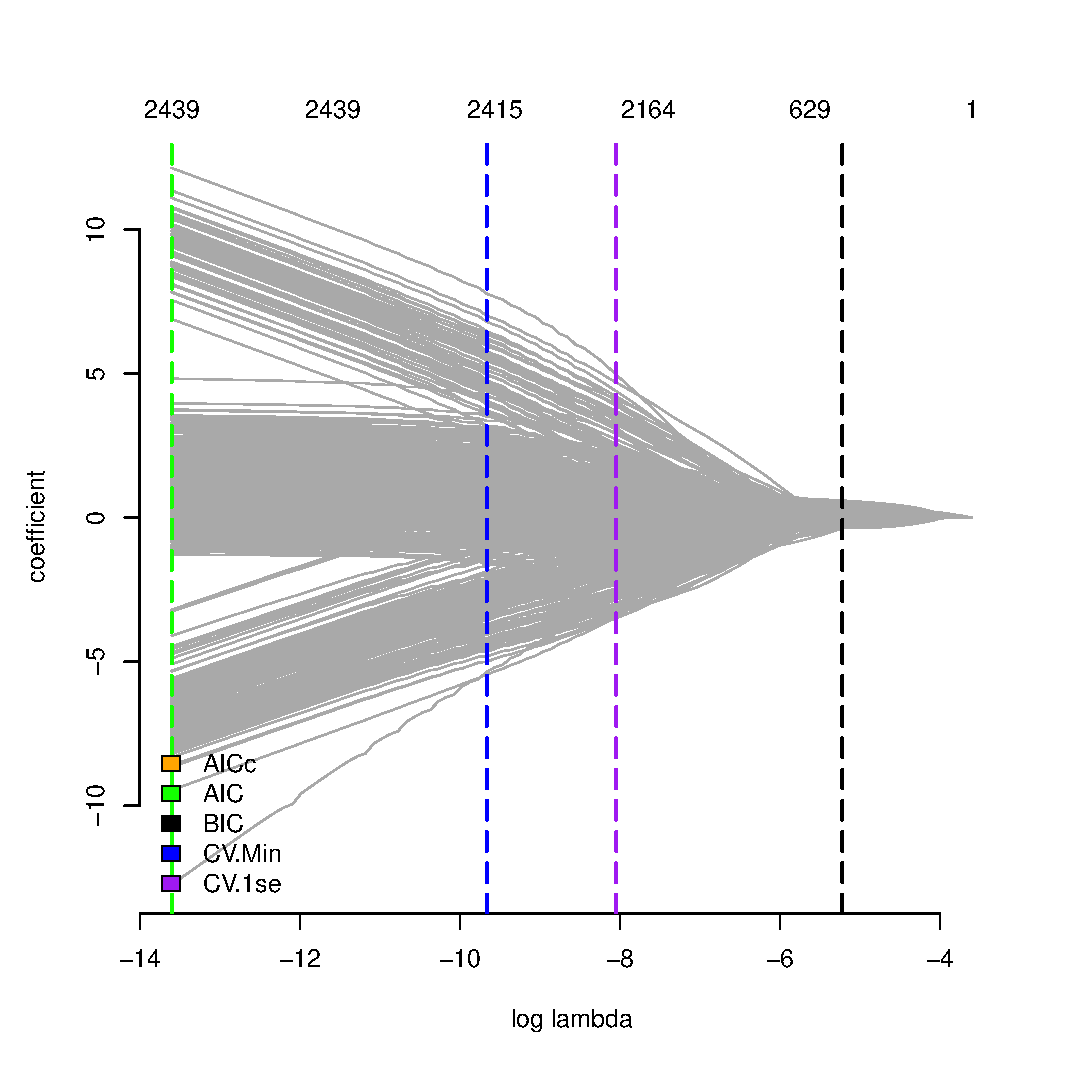
\includegraphics[width=\textwidth]{ic_pl_nhl_c.eps}
    \caption{Gamma-Lasso Path Plot with ICs}
    \label{fig:pl_ic_nhl}
  \end{subfigure}
  \caption{CV and Gamma-Lasso Results for Simplified Model}
\end{figure}

\begin{figure}[!htb]
  \centering
  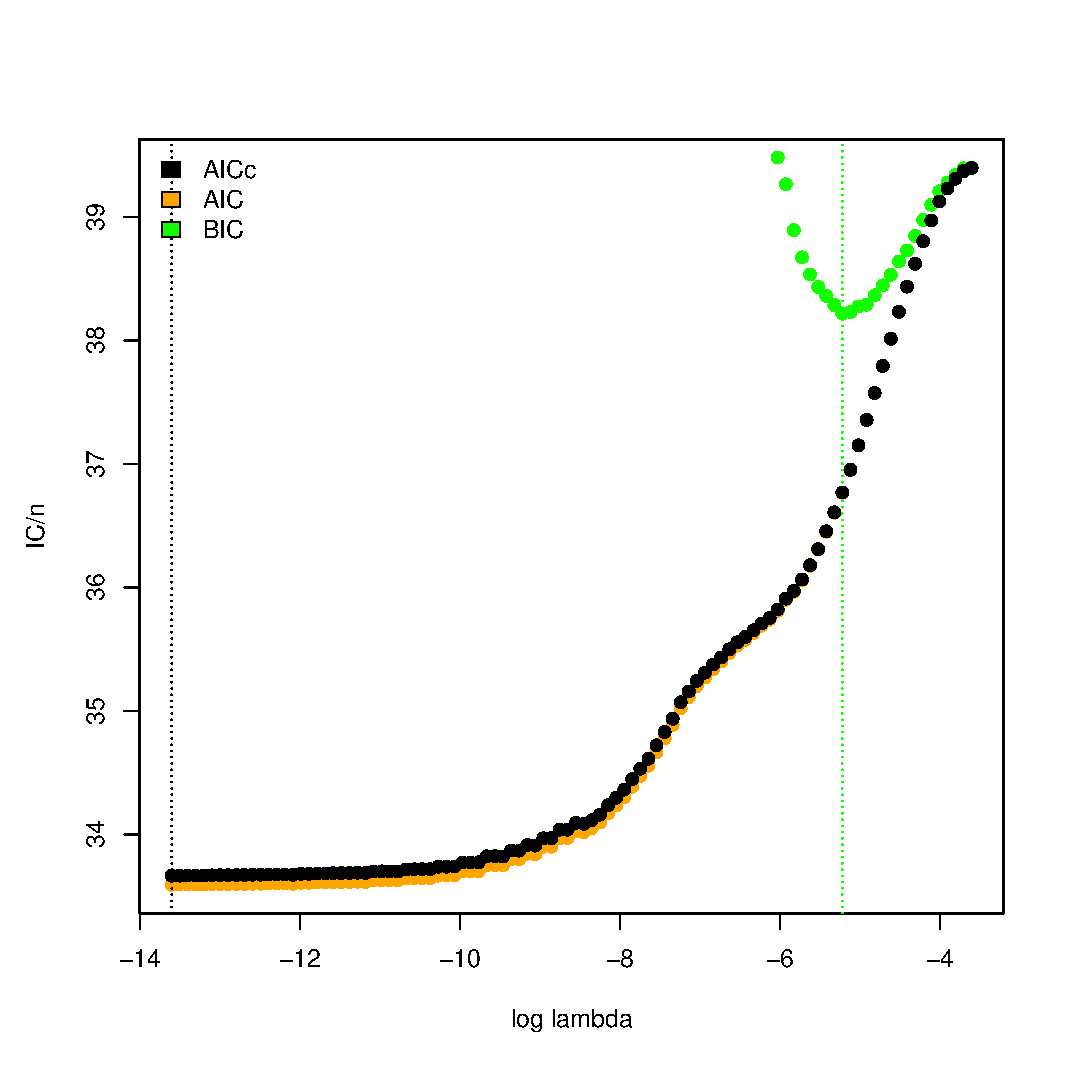
\includegraphics[scale=.5]{ic_pl_nhl_b.eps}
  \caption{Gamma-Lasso with ICs}
  \label{fig:pl_ic_nhl_b}
\end{figure}

\section{Comparison to Classic Plus-Minus}

The player coefficients in our model account for probabilities on a per-goal basis, while the classic plus-minus statistic is an additive function of the net number of goals scored while a player is on the ice. We can use our model to construct something like an adjusted plus-minus, and we can answer the following question: what is the plus-minus that a player should be given credit for? Our adjusted plus-minus can answer this question because it is based on the player-specific probabilities of goals scored.

The player coefficients described in Section 1 describe the odds multiplier that a goal scored while player is on the ice. First, we convert this odds multiplier into a probability:
\[ p_j = \frac{1}{1+\exp \left(-\beta_j\right)} \]
For each player, we count \textbf{G}, the number of goals scored (for any team) while that player was on the ice. Our expectation of the number of goals scored by that players team is therefore $G p_j$ and the number of goals scored against his team is $G (1-p_j)$. The player's adjusted plus-minus is the sum of these two:
\begin{align*} 
PM_{adj} & = G p_j + G (1-p_j) \\
 & = G (2 p_j - 1)
\end{align*}
This adjusted plus-minus stat can be interpreted on the same scale as classic plus-minus. In Figure~\ref{fig:pm_compare}, we plot our adjusted plus-minus against the classic plus-minus statistic to see how they compare. We can say that the stats ``agree'' on a player if the player is in quadrant 1 or quadrant 3 (i.e. both stats give the player a positive or a negative rating). Of the 646 players in our sample (those for which their player coefficients in the original model are non-zero), the statistics only agree on 375 of them, or around 58 percent of the sample. This lends some credence to the belief in the analytics community that classic plus minus really is a ``horse s***'' statistic\footnote{Colorful quote courtesy of NHL executive Brian Burke in an interview with the Edmonton Journal (http://blogs.edmontonjournal.com/2013/05/13/just-how-horse-shit-is-the-nhls-official-plus-minus-stat/)}.

\begin{figure}[!htb]
  \centering
  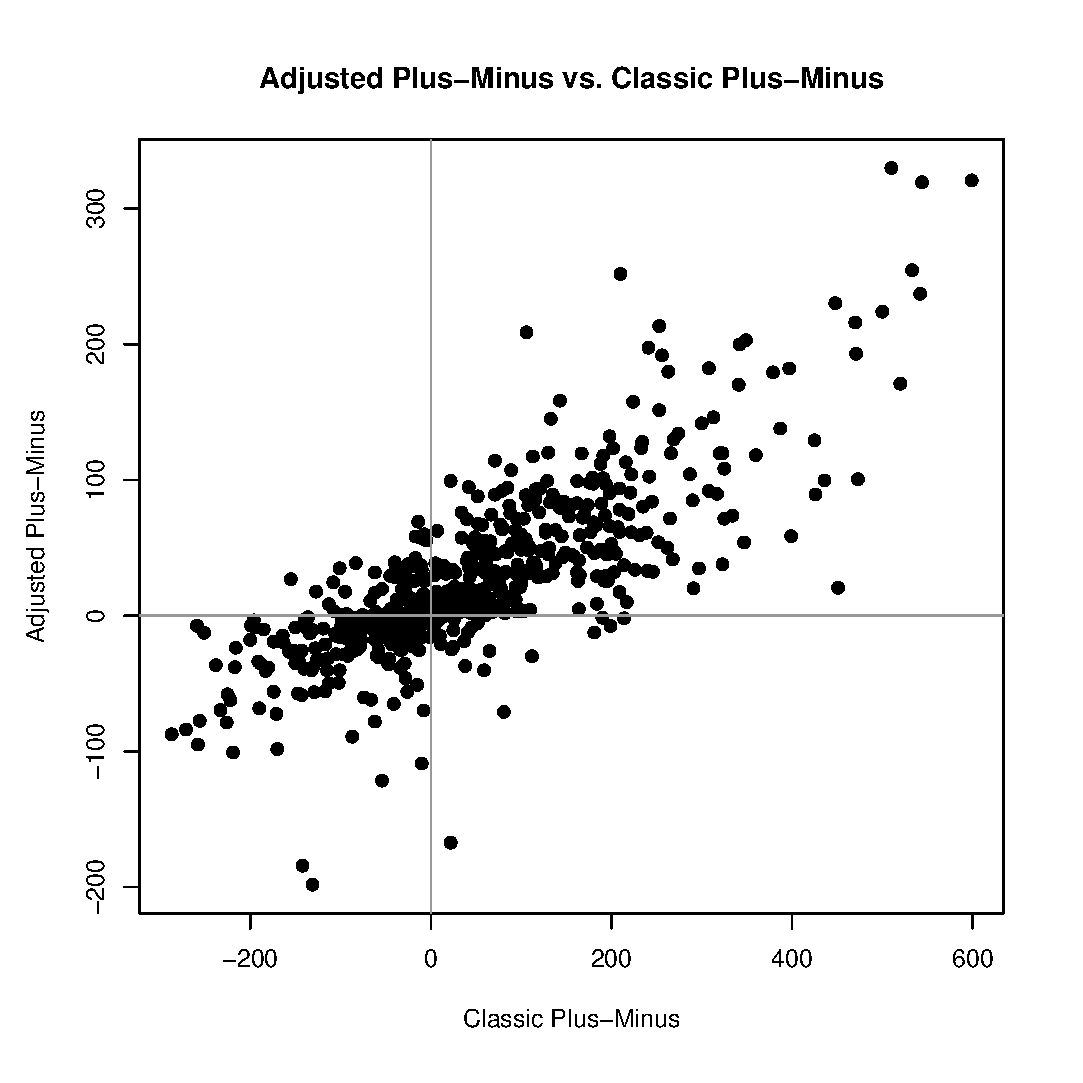
\includegraphics[scale=.5]{pm_compare.eps}
  \caption{Plus-Minus Stat Comparison}
  \label{fig:pm_compare}
\end{figure}

\end{document}
